\documentclass[journal,12pt,twocolumn]{IEEEtran}

\usepackage{setspace}
\usepackage{gensymb}

\singlespacing


\usepackage[cmex10]{amsmath}

\usepackage{amsthm}

\usepackage{mathrsfs}
\usepackage{txfonts}
\usepackage{stfloats}
\usepackage{bm}
\usepackage{cite}
\usepackage{cases}
\usepackage{subfig}

\usepackage{longtable}
\usepackage{multirow}

\usepackage{enumitem}
\usepackage{mathtools}
\usepackage{steinmetz}
\usepackage{tikz}
\usepackage{circuitikz}
\usepackage{verbatim}
\usepackage{tfrupee}
\usepackage[breaklinks=true]{hyperref}
\usepackage{graphicx}
\usepackage{tkz-euclide}
\usepackage{float}

\usetikzlibrary{calc,math}
\usepackage{listings}
    \usepackage{color} %%
    \usepackage{array} %%
    \usepackage{longtable} %%
    \usepackage{calc} %%
    \usepackage{multirow} %%
    \usepackage{hhline} %%
    \usepackage{ifthen} %%
    \usepackage{lscape}     
\usepackage{multicol}
\usepackage{chngcntr}
\newcommand{\norm}[1]{\left\lVert#1\right\rVert}

\DeclareMathOperator*{\Res}{Res}

\renewcommand\thesection{\arabic{section}}
\renewcommand\thesubsection{\thesection.\arabic{subsection}}
\renewcommand\thesubsubsection{\thesubsection.\arabic{subsubsection}}

\renewcommand\thesectiondis{\arabic{section}}
\renewcommand\thesubsectiondis{\thesectiondis.\arabic{subsection}}
\renewcommand\thesubsubsectiondis{\thesubsectiondis.\arabic{subsubsection}}


\hyphenation{op-tical net-works semi-conduc-tor}
\def\inputGnumericTable{} %%

\lstset{
%language=C,
frame=single, 
breaklines=true,
columns=fullflexible
}
\begin{document}


\newtheorem{theorem}{Theorem}[section]
\newtheorem{problem}{Problem}
\newtheorem{proposition}{Proposition}[section]
\newtheorem{lemma}{Lemma}[section]
\newtheorem{corollary}[theorem]{Corollary}
\newtheorem{example}{Example}[section]
\newtheorem{definition}[problem]{Definition}

\newcommand{\BEQA}{\begin{eqnarray}}
\newcommand{\EEQA}{\end{eqnarray}}
\newcommand{\define}{\stackrel{\triangle}{=}}
\newcommand\hlight[1]{\tikz[overlay, remember picture,baseline=-\the\dimexpr\fontdimen22\textfont2\relax]\node[rectangle,fill=blue!50,rounded corners,fill opacity = 0.2,draw,thick,text opacity =1] {$#1$};}
\bibliographystyle{IEEEtran}
\providecommand{\mbf}{\mathbf}
\providecommand{\pr}[1]{\ensuremath{\Pr\left(#1\right)}}
\providecommand{\qfunc}[1]{\ensuremath{Q\left(#1\right)}}
\providecommand{\sbrak}[1]{\ensuremath{{}\left[#1\right]}}
\providecommand{\lsbrak}[1]{\ensuremath{{}\left[#1\right.}}
\providecommand{\rsbrak}[1]{\ensuremath{{}\left.#1\right]}}
\providecommand{\brak}[1]{\ensuremath{\left(#1\right)}}
\providecommand{\lbrak}[1]{\ensuremath{\left(#1\right.}}
\providecommand{\rbrak}[1]{\ensuremath{\left.#1\right)}}
\providecommand{\cbrak}[1]{\ensuremath{\left\{#1\right\}}}
\providecommand{\lcbrak}[1]{\ensuremath{\left\{#1\right.}}
\providecommand{\rcbrak}[1]{\ensuremath{\left.#1\right\}}}
\theoremstyle{remark}
\newtheorem{rem}{Remark}
\newcommand{\sgn}{\mathop{\mathrm{sgn}}}
%\providecommand{\abs}[1]{\left\vert#1\right\vert}
\providecommand{\res}[1]{\Res\displaylimits_{#1}} 
\providecommand{\norm}[1]{$\left\lVert#1\right\rVert$}
%\providecommand{\norm}[1]{\lVert#1\rVert}
\providecommand{\mtx}[1]{\mathbf{#1}}
%\providecommand{\mean}[1]{E\left[ #1 \right]}
\providecommand{\fourier}{\overset{\mathcal{F}}{ \rightleftharpoons}}
%\providecommand{\hilbert}{\overset{\mathcal{H}}{ \rightleftharpoons}}
\providecommand{\system}{\overset{\mathcal{H}}{ \longleftrightarrow}}
 %\newcommand{\solution}[2]{\textbf{Solution:}{#1}}
\newcommand{\solution}{\noindent \textbf{Solution: }}
\newcommand{\cosec}{\,\text{cosec}\,}
\providecommand{\dec}[2]{\ensuremath{\overset{#1}{\underset{#2}{\gtrless}}}}
\newcommand{\myvec}[1]{\ensuremath{\begin{pmatrix}#1\end{pmatrix}}}
\newcommand{\mydet}[1]{\ensuremath{\begin{vmatrix}#1\end{vmatrix}}}
\numberwithin{equation}{subsection}
\makeatletter
\@addtoreset{figure}{problem}
\makeatother
\let\StandardTheFigure\thefigure
\let\vec\mathbf
\renewcommand{\thefigure}{\theproblem}
\def\putbox#1#2#3{\makebox[0in][l]{\makebox[#1][l]{}\raisebox{\baselineskip}[0in][0in]{\raisebox{#2}[0in][0in]{#3}}}}
     \def\rightbox#1{\makebox[0in][r]{#1}}
     \def\centbox#1{\makebox[0in]{#1}}
     \def\topbox#1{\raisebox{-\baselineskip}[0in][0in]{#1}}
     \def\midbox#1{\raisebox{-0.5\baselineskip}[0in][0in]{#1}}
\vspace{3cm}
\title{Assignment No.3}
\author{Panisha Gundelli}
\maketitle
\newpage
\bigskip
\renewcommand{\thefigure}{\theenumi}
\renewcommand{\thetable}{\theenumi}
Download latex-tikz codes from
\begin{lstlisting}
https://github.com/Panisha707/ASSIGNMENT03/blob/main/main.tex
\end{lstlisting}
%
Download python codes from
\begin{lstlisting}
https://github.com/Panisha707/ASSIGNMENT03/blob/main/untitled21.py
\end{lstlisting}
%
Question taken from
\begin{lstlisting}
Construction, Excercise 2.5
\end{lstlisting}
\section{Question No 1}
Construct LIFT such that LI=4, IF=3, TL=2.5, LF=4.5, IT=4
\section{Solution}
Let,there are two triangles $\triangle FLI$ and $\triangle TLI$\\
In $\triangle FLI$
\begin{align}
  \norm{\vec{L}-\vec{I}}+\norm{\vec{I}-\vec{F}}=7 > \norm{\vec{L}-\vec{F}}
\end{align}
\begin{align}
   \norm{\vec{L}-\vec{F}}+\norm{\vec{I}-\vec{F}}=7.5 > \norm{\vec{L}-\vec{I}} 
\end{align}
\begin{align}
    \norm{\vec{L}-\vec{F}}+\norm{\vec{L}-\vec{I}}=8.5 > \norm{\vec{I}-\vec{F}}
\end{align}
triangle inequality is satisfied. Similarly \\
In $\triangle TLI$
\begin{align}
  \norm{\vec{L}-\vec{I}}+\norm{\vec{I}-\vec{T}}=8 > \norm{\vec{T}-\vec{L}}
\end{align}
\begin{align}
   \norm{\vec{L}-\vec{I}}+\norm{\vec{T}-\vec{L}}=6.5 > \norm{\vec{I}-\vec{T}} 
\end{align}
\begin{align}
   \norm{\vec{I}-\vec{T}}+\norm{\vec{T}-\vec{L}}=6.5 > \norm{\vec{L}-\vec{I}} 
\end{align}
and triangle inequaliity is satisfied.
$\therefore$ the given sides form a quadrilateral.\\
\\The vertices of the quadrilateral are calculated by taking $\triangle FLI$ and $\triangle TLI$\\
\\From $\triangle FLI$,let the side of the triangle are
\begin{center}
   a=4, b=3, c=4.5 
\end{center}
Let the vertices of the triangle 
\begin{center}
   $\vec{F}=\myvec{p\\q}, \vec{L}=\myvec{0\\0}, \vec{I}=\myvec{a\\0}$ 
\end{center}
\begin{align}
    \vec{F}=c\myvec{\cos \theta\\\sin \theta}
\end{align}
\\ we use law of cosines
\begin{align}
   \cos\theta=\frac{a^2+c^2-b^2}{2ac}
\end{align}
\begin{align}
    =\frac{4^2+4.5^2-3^2}{2\times4\times4.5}
\end{align}
\begin{align}
     =0.7569
\end{align}
\begin{align}
    \implies \theta=40.808
\end{align}
\\Thus,
\begin{align}
   \vec{F}=4.5\myvec{\cos40.808\\\sin40.808} 
\end{align}
\begin{align}
    \vec{F}=4.5\myvec{0.7569\\0.6535} 
\end{align}
\begin{align}
    \vec{F}=\myvec{3.406\\2.940} 
\end{align}
The vertices of the $\triangle FLI$ are found out to be\\
\begin{align}
    \vec{F}=\myvec{3.406\\2.940}, \vec{L}=\myvec{0\\0}, \vec{I}=\myvec{4\\0}
\end{align}
\\From $\triangle TLI$,let the sides of the triangle
\begin{center}
   a=4, b=4, c=2.5 
\end{center}
Let the vertices of the triangle 
\begin{center}
   $\vec{T}=\myvec{p\\q}, \vec{L}=\myvec{0\\0}, \vec{I}=\myvec{a\\0}$ 
\end{center}
\begin{align}
    \vec{T}=c\myvec{\cos \theta\\\sin \theta}
\end{align}
 we use law of cosines
\begin{align}
   \cos\theta=\frac{a^2+c^2-b^2}{2ac}
\end{align}
\begin{align}
    =\frac{4^2+2.5^2-4^2}{2\times4\times2.5}
\end{align}
\begin{align}
    =0.3125
\\
    \implies \theta=71.790
\end{align}
Thus
\begin{align}
   \vec{T}=2.5\myvec{\cos71.790\\\sin71.790} 
\end{align}
\begin{align}
    \vec{T}=2.5\myvec{0.3125\\0.9499} 
\end{align}
\begin{align}
    \vec{T}=\myvec{0.781\\2.374} 
\end{align}
The vertices of the $\triangle TLI$ are found out to be
\begin{align}
    \vec{T}=\myvec{0.781\\2.374}, \vec{L}=\myvec{0\\0}, \vec{I}=\myvec{4\\0}
\end{align}
$\therefore$The vertices of the quadrilateral LIFT can be written as
\begin{align}
   \vec{L}=\myvec{0\\0}, \vec{I}=\myvec{4\\0},\vec{F}=\myvec{3.406\\2.940}, \vec{T}=\myvec{0.781\\2.374}
\end{align}
$\therefore$ Fig.\ref{Graphical solution}  verifies that the points can form a quadrilateral.
   \numberwithin{figure}{section}
\begin{figure}[ht]
    \centering
    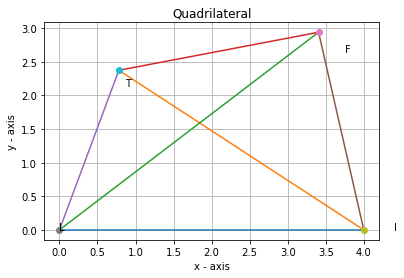
\includegraphics[width=\columnwidth]{quadrilateral.png}
    \caption{Quadrilateral LIFT}
    \label{Graphical solution}
\end{figure}
\end{document}
